% questions.tex —— 2008 年·普通高等学校招生考试·安徽卷·理科 · 题目内容片段（无答案）
% 由 tools/generate_projects.py 依来源总账自 2008/2008_数学真题_安徽理_试题.md 生成，勿手改（改源 MD 后重跑）


\gkpart{一、选择题}

\begin{question}
\gkti{1}复数 $\mathrm i^3(1+\mathrm i)^2=$（　）

（A）$2$

（B）$-2$

（C）$2\mathrm i$

（D）$-2\mathrm i$

\end{question}
\begin{question}
\gkti{2}集合 $A=\{y\in\mathbf R\mid y=\lg x,\ x>1\}$，$B=\{-2,-1,1,2\}$，则下列结论正确的是（　）

（A）$A\cap B=\{-2,-1\}$

（B）$(\complement_{\mathbf R}A)\cup B=(-\infty,0)$

（C）$A\cup B=(0,+\infty)$

（D）$(\complement_{\mathbf R}A)\cap B=\{-2,-1\}$

\end{question}
\begin{question}
\gkti{3}在平行四边形 $ABCD$ 中，$AC$ 为一条对角线，若 $\overrightarrow{AB}=(2,4)$，$\overrightarrow{AC}=(1,3)$，则 $\overrightarrow{BD}=$（　）

（A）$(-2,-4)$

（B）$(-3,-5)$

（C）$(3,5)$

（D）$(2,4)$

\end{question}
\begin{question}
\gkti{4}已知 $m$，$n$ 是两条不同直线，$\alpha$，$\beta$，$\gamma$ 是三个不同平面，下列命题中正确的是（　）

（A）若 $m\parallel\alpha$，$n\parallel\alpha$，则 $m\parallel n$

（B）若 $\alpha\perp\gamma$，$\beta\perp\gamma$，则 $\alpha\parallel\beta$

（C）若 $m\parallel\alpha$，$m\parallel\beta$，则 $\alpha\parallel\beta$

（D）若 $m\perp\alpha$，$n\perp\alpha$，则 $m\parallel n$

\end{question}
\begin{question}
\gkti{5}将函数 $y=\sin\left(2x+\dfrac{\pi}{3}\right)$ 的图象按向量 $\boldsymbol a$ 平移后所得的图象关于点 $\left(-\dfrac{\pi}{12},0\right)$ 中心对称，则向量 $\boldsymbol a$ 的坐标可能为（　）

（A）$\left(-\dfrac{\pi}{12},0\right)$

（B）$\left(-\dfrac{\pi}{6},0\right)$

（C）$\left(\dfrac{\pi}{12},0\right)$

（D）$\left(\dfrac{\pi}{6},0\right)$

\end{question}
\begin{question}
\gkti{6}设 $(1+x)^8=a_0+a_1x+\cdots+a_8x^8$，则 $a_0$，$a_1$，$\cdots$，$a_8$ 中奇数的个数为（　）

（A）$2$

（B）$3$

（C）$4$

（D）$5$

\end{question}
\begin{question}
\gkti{7}$a<0$ 是方程 $ax^2+2x+1=0$ 至少有一个负数根的（　）

（A）必要不充分条件

（B）充分不必要条件

（C）充分必要条件

（D）既不充分也不必要条件

\end{question}
\begin{question}
\gkti{8}若过点 $A(4,0)$ 的直线 $l$ 与曲线 $(x-2)^2+y^2=1$ 有公共点，则直线 $l$ 的斜率的取值范围为（　）

（A）$[-\sqrt3,\sqrt3]$

（B）$(-\sqrt3,\sqrt3)$

（C）$\left[-\dfrac{\sqrt3}{3},\dfrac{\sqrt3}{3}\right]$

（D）$\left(-\dfrac{\sqrt3}{3},\dfrac{\sqrt3}{3}\right)$

\end{question}
\begingroup
\renewenvironment{question}{\Needspace{0.48\textheight}}{}
\begin{question}
\gkti{9}在同一平面直角坐标系中，函数 $y=g(x)$ 的图象与 $y=\mathrm e^x$ 的图象关于直线 $y=x$ 对称。而函数 $y=f(x)$ 的图象与 $y=g(x)$ 的图象关于 $y$ 轴对称。若 $f(m)=-1$，则 $m$ 的值是（　）

（A）$-\mathrm e$

（B）$-\dfrac1{\mathrm e}$

（C）$\mathrm e$

（D）$\dfrac1{\mathrm e}$

\Needspace{0.4\textheight}
\end{question}
\endgroup
\begin{question}
\gkti{10}设两个正态分布 $N(\mu_1,\sigma_1^2)$（$\sigma_1>0$）和 $N(\mu_2,\sigma_2^2)$（$\sigma_2>0$）的密度函数图象如图所示，则有（　）
\nopagebreak[4]
\begin{center}% 2008 年安徽卷理科第 10 题：两个正态分布 N(μ1,σ1²)、N(μ2,σ2²) 的密度函数图象。
% 来源 PDF：gaokaomath-src/普通高考/2008/2008安徽理.pdf
% SHA-256：3493c8cb26596a78dafa0c1169fbdbfa4e69d8e593193f7c47128763b095c564
% 原页：2008安徽理.pdf 第 1 页（A3 三栏）第 2 栏，书页码 421。
% 重绘依据：按原页峰位与峰高重绘：源图左侧曲线峰约在 x=-0.28、高约 1.4（σ 较小），
%   右侧曲线峰约在 x=0.26、高约 0.85（σ 较大），本图取 μ1=-0.3、μ2=0.3 与之对齐；
%   坐标轴刻度 -1、-0.5、0、0.5、1 与 0.2～1.4 照原页。
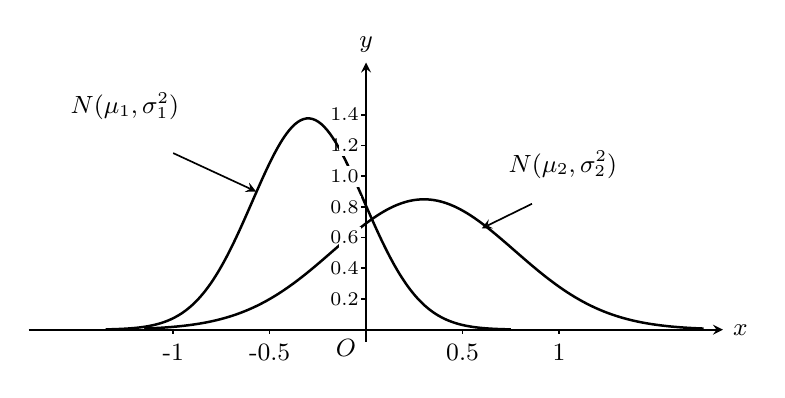
\begin{tikzpicture}[x=2.45cm, y=1.95cm, semithick, font=\small]
  \draw[->,>=stealth] (-1.75,0) -- (1.85,0) node[right] {$x$};
  \draw[->,>=stealth] (0,-0.08) -- (0,1.74) node[above] {$y$};
  \node[below left] at (0,0) {$O$};

  \foreach \x/\lab in {-1/-1, -0.5/-0.5, 0.5/0.5, 1/1} {
    \draw (\x,0) -- (\x,-0.03);
    \node[below] at (\x,-0.03) {\lab};
  }

  % 左：N(μ1,σ1²)，μ1≈-0.3，σ1≈0.29
  \draw[line width=0.9pt, domain=-1.35:0.75, samples=140]
    plot (\x, {1.376*exp(-((\x+0.3)*(\x+0.3))/(2*0.29*0.29))});
  % 右：N(μ2,σ2²)，μ2≈0.3，σ2≈0.47
  \draw[line width=0.9pt, domain=-1.15:1.75, samples=140]
    plot (\x, {0.849*exp(-((\x-0.3)*(\x-0.3))/(2*0.47*0.47))});

  \node[above] at (-1.25,1.30) {$N(\mu_1,\sigma_1^2)$};
  \draw[->,>=stealth] (-1.00,1.15) -- (-0.57,0.90);
  \node[above] at (1.02,0.92) {$N(\mu_2,\sigma_2^2)$};
  \draw[->,>=stealth] (0.86,0.82) -- (0.60,0.66);

  % 纵轴刻度与数字置于曲线之后，并以白色底遮断曲线，避免数字被曲线穿压
  \foreach \y in {0.2,0.4,0.6,0.8,1.0,1.2,1.4} {
    \draw (0,\y) -- (-0.03,\y);
    \fill[white] (-0.138,\y-0.068) rectangle (-0.028,\y+0.068);
    \node[left, inner sep=0.3pt, font=\scriptsize] at (-0.03,\y) {\y};
  }
\end{tikzpicture}
\end{center}
\nopagebreak[4]
（A）$\mu_1<\mu_2$，$\sigma_1<\sigma_2$

（B）$\mu_1<\mu_2$，$\sigma_1>\sigma_2$

（C）$\mu_1>\mu_2$，$\sigma_1<\sigma_2$

（D）$\mu_1>\mu_2$，$\sigma_1>\sigma_2$

\end{question}
\begin{question}
\gkti{11}若函数 $f(x)$，$g(x)$ 分别是 $\mathbf R$ 上的奇函数、偶函数，且满足 $f(x)-g(x)=\mathrm e^x$，则有（　）

（A）$f(2)<f(3)<g(0)$

（B）$g(0)<f(3)<f(2)$

（C）$f(2)<g(0)<f(3)$

（D）$g(0)<f(2)<f(3)$

\end{question}
\begin{question}
\gkti{12}$12$ 名同学合影，站成前排 $4$ 人后排 $8$ 人，现摄影师要从后排 $8$ 人中抽 $2$ 人调整到前排，若其他人的相对顺序不变，则不同调整方法的总数是（　）

（A）$\mathrm C_8^2\mathrm A_3^2$

（B）$\mathrm C_8^2\mathrm A_6^6$

（C）$\mathrm C_8^2\mathrm A_6^2$

（D）$\mathrm C_8^2\mathrm A_5^2$

\end{question}
\gkpart{二、填空题}

\begin{question}
\gkti{13}函数 $f(x)=\dfrac{\sqrt{|x-2|-1}}{\log_2(x-1)}$ 的定义域为\gkblank{}。

\end{question}
\begingroup
\renewenvironment{question}{\Needspace{0.46\textheight}}{}
\begin{question}
\gkti{14}在数列 $\{a_n\}$ 中，$a_n=4n-\dfrac52$，$a_1+a_2+\cdots+a_n=an^2+bn$，$n\in\mathbf N^*$，其中 $a$，$b$ 为常数，则 $\lim\limits_{n\to\infty}\dfrac{a^n-b^n}{a^n+b^n}$ 的值是\gkblank{}。

\end{question}
\endgroup
\begin{question}
\gkti{15}若 $A$ 为不等式组 $\begin{cases}x\leqslant0,\\ y\geqslant0,\\ y-x\leqslant2\end{cases}$ 表示的平面区域，则当 $a$ 从 $-2$ 连续变化到 $1$ 时，动直线 $x+y=a$ 扫过 $A$ 中的那部分区域的面积为\gkblank{}。

\end{question}
\begin{question}
\gkti{16}已知 $A$，$B$，$C$，$D$ 在同一个球面上，$AB\perp$ 平面 $BCD$，$BC\perp CD$，若 $AB=6$，$AC=2\sqrt{13}$，$AD=8$，则 $B$，$C$ 两点间的球面距离是\gkblank{}。

\end{question}
\gkpart{三、解答题}

\begingroup
\renewenvironment{question}{\Needspace{0.46\textheight}}{}
\begin{question}
\gkti{17}已知函数 $f(x)=\cos\left(2x-\dfrac{\pi}{3}\right)+2\sin\left(x-\dfrac{\pi}{4}\right)\sin\left(x+\dfrac{\pi}{4}\right)$。

（1）求函数 $f(x)$ 的最小正周期和图象的对称轴方程；

（2）求函数 $f(x)$ 在区间 $\left[-\dfrac{\pi}{12},\dfrac{\pi}{2}\right]$ 上的值域。

\Needspace{0.4\textheight}
\end{question}
\endgroup
\begin{question}
\gkti{18}如图，在四棱锥 $O-ABCD$ 中，底面 $ABCD$ 是边长为 $1$ 的菱形，$\angle ABC=\dfrac{\pi}{4}$。$OA\perp$ 底面 $ABCD$，$OA=2$，$M$ 为 $OA$ 的中点，$N$ 为 $BC$ 的中点。

（1）证明：直线 $MN\parallel$ 平面 $OCD$；

（2）求异面直线 $AB$ 与 $MD$ 所成角的大小；

（3）求点 $B$ 到平面 $OCD$ 的距离。
\nopagebreak[4]
\begin{center}% 2008 年安徽卷理科第 18 题：四棱锥 O-ABCD，底面菱形边长 1，∠ABC=π/4，
%   OA⊥底面，OA=2，M 为 OA 中点，N 为 BC 中点。
% 来源 PDF：gaokaomath-src/普通高考/2008/2008安徽理.pdf
% SHA-256：3493c8cb26596a78dafa0c1169fbdbfa4e69d8e593193f7c47128763b095c564
% 原页：2008安徽理.pdf 第 1 页（A3 三栏）第 3 栏，书页码 421。
% 重绘依据：按原页斜投影重绘：A 为被遮挡的后顶点，B 在左前、C 在右前、D 在右后；
%   A—B、A—D、A—O 用虚线，M、N 分别为 OA、BC 的中点，连 M—N、M—D 虚线。
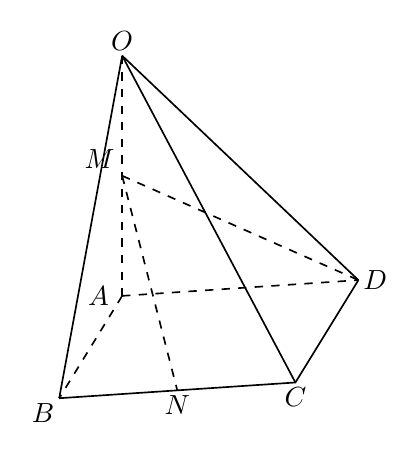
\begin{tikzpicture}[scale=1.0, semithick,
  every node/.style={inner sep=1.5pt}]

  \coordinate (B) at (0.40,0.75);
  \coordinate (C) at (3.40,0.95);
  \coordinate (D) at (4.20,2.25);
  \coordinate (A) at (1.20,2.05);
  \coordinate (O) at (1.20,5.10);
  \coordinate (M) at (1.20,3.575);
  \coordinate (N) at (1.90,0.85);

  % 底面：前棱与右棱可见，后两条棱被遮挡
  \draw (B) -- (C) -- (D);
  \draw[dashed] (A) -- (B);
  \draw[dashed] (A) -- (D);

  % 侧棱
  \draw (O) -- (B);
  \draw (O) -- (C);
  \draw (O) -- (D);
  \draw[dashed] (O) -- (A);

  % M 为 OA 中点，N 为 BC 中点
  \draw[dashed] (M) -- (N);
  \draw[dashed] (M) -- (D);

  \node[above] at (O) {$O$};
  \node[above left=1pt] at (M) {$M$};
  \node[left=3pt] at (A) {$A$};
  \node[below left] at (B) {$B$};
  \node[below] at (C) {$C$};
  \node[right] at (D) {$D$};
  \node[below] at (N) {$N$};
\end{tikzpicture}
\end{center}
\nopagebreak[4]
\end{question}
\begin{question}
\gkti{19}为防止风沙危害，某地决定建设防护绿化带，种植杨树、沙柳等植物。某人一次种植了 $n$ 株沙柳，各株沙柳成活与否是相互独立的，成活率为 $p$，设 $\xi$ 为成活沙柳的株数，数学期望 $E\xi=3$，标准差 $\sigma\xi$ 为 $\dfrac{\sqrt6}{2}$。

（1）求 $n$，$p$ 的值，并写出 $\xi$ 的分布列；

（2）若有 $3$ 株或 $3$ 株以上的沙柳未成活，则需要补种，求需要补种沙柳的概率。

\end{question}
\begin{question}
\gkti{20}设函数 $f(x)=\dfrac1{x\ln x}$（$x>0$ 且 $x\neq1$）。

（1）求函数 $f(x)$ 的单调区间；

（2）已知 $2^{\frac1x}>x^a$ 对任意 $x\in(0,1)$ 成立，求实数 $a$ 的取值范围。

\end{question}
\begin{question}
\gkti{21}设数列 $\{a_n\}$ 满足 $a_0=0$，$a_{n+1}=ca_n^3+1-c$，$n\in\mathbf N^*$，其中 $c$ 为实数。

（1）证明：$a_n\in[0,1]$ 对任意 $n\in\mathbf N^*$ 成立的充分必要条件是 $c\in[0,1]$；

（2）设 $0<c<\dfrac13$，证明：$a_n\geqslant1-(3c)^{n-1}$，$n\in\mathbf N^*$；

（3）设 $0<c<\dfrac13$，证明：$a_1^2+a_2^2+\cdots+a_n^2>n+1-\dfrac{2}{1-3c}$，$n\in\mathbf N^*$。

\end{question}
\begin{question}
\gkti{22}设椭圆 $C$：$\dfrac{x^2}{a^2}+\dfrac{y^2}{b^2}=1$（$a>b>0$）过点 $M(\sqrt2,1)$，且左焦点为 $F_1(-\sqrt2,0)$。

（1）求椭圆 $C$ 的方程；

（2）当过点 $P(4,1)$ 的动直线 $l$ 与椭圆 $C$ 相交于两不同点 $A$，$B$ 时，在线段 $AB$ 上取点 $Q$，满足 $\left|\overrightarrow{AP}\right|\cdot\left|\overrightarrow{QB}\right|=\left|\overrightarrow{AQ}\right|\cdot\left|\overrightarrow{PB}\right|$，证明：点 $Q$ 总在某定直线上。

\end{question}